\documentclass[../../main.tex]{subfiles}

\begin{document}
En problemas de clasificación binaria, existen diferentes métricas para evaluar el
desempeño del modelo utilizado, siempre sobre el conjunto de test. Las que más relevancia
tendrán depende del contexto del problema. Para describirlas, utilizaremos la siguiente
notación, asumiendo que la etiqueta 1 corresponde a la clase ``positiva'' y la 0 a la
``negativa'':
\begin{itemize}
    \item \(VP\): Verdaderos Positivos. Es la cantidad de predicciones correctas para la
    clase positiva. Es decir, son aquellas observaciones cuya etiqueta verdadera es 1 y
    que el modelo también clasificó como 1. En nuestro caso, los \(VP\) son los indiviudos
    de control que el modelo identificó correctamente como tales.
    \item \(VN\): Verdaderos Negativos. Es la cantidad de predicciones correctas para la
    clase negativa. Es decir, son aquellas observaciones cuya etiqueta verdadera es 0 y
    que el modelo también clasificó como 0. En nuestro caso, los \(VN\) son los indiviudos
    NiNi que el modelo identificó correctamente como tales.
    \item \(FP\): Falsos Positivos. Es la cantidad de predicciones incorrectas para la
    clase negativa. Es decir, son aquellas observaciones cuya etiqueta verdadera es 0 pero
    que el modelo clasificó como 1. En nuestro caso, los \(FP\) son los indiviudos NiNi
    que el modelo identificó incorrectamente como de control.
    \item \(FN\): Falsos Negativos. Es la cantidad de predicciones incorrectas para la
    clase positiva. Es decir, son aquellas observaciones cuya etiqueta verdadera es 1 pero
    que el modelo clasificó como 0. En nuestro caso, los \(FN\) son los indiviudos de
    control que el modelo identificó incorrectamente como NiNi.
\end{itemize}

Todas estas cantidades se suelen presentar de forma conjunta en lo que se denomina
\textbf{matriz de confusión}, cuya representación se encuentra en la Figura
\ref{fig:confusion-matrix}.

\begin{figure}[H]
    \centering
    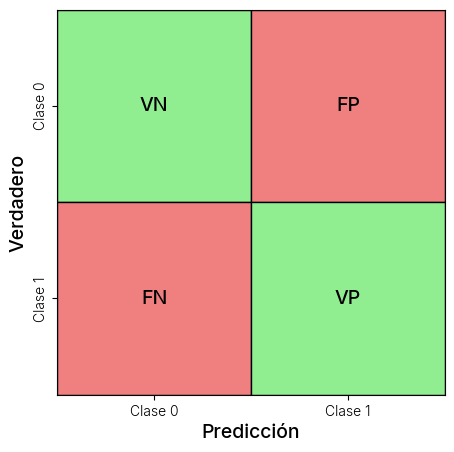
\includegraphics[width=0.4\textwidth]{figs/matriz-confusion.png}
    \caption{Matriz de confusión.}
    \label{fig:confusion-matrix}
\end{figure}

Con estos conceptos en mente, algunas de las métricas que se suelen considerar son las
siguientes, cuyo valor mínimo es 0 y el máximo es 1, y se pueden calcular tanto para la
clase positiva como la negativa (en las explicaciones, asumimos que se calculan sobre la
positiva):

\subsection{Exactitud}
Es la proporción de entradas para las cuales el modelo predijo la salida correcta.
Su fórmula está dada por:
\[
    Exactitud = \frac{VP + VN}{VP + VN + FP + FN}
\]

Utilizar esta medida no es recomendable en datasets desbalanceados, es decir en aquellos
en donde hay un alto porcentaje de una clase pero bajo de otra. Veamos por qué con un
ejemplo.

Supongamos que tenemos un dataset de 100 muestras en donde el 90\% de los datos tienen
etiqueta 0 y el restante 10\% tiene etiqueta 1. Se puede ver que si el modelo predice un
valor de 0 para cualquier entrada, entonces tendría una exactitud del 90\%, que es un
porcentaje bastante alto, pero se habrá equivocado en todas las instancias positivas.
Por esto, suele ser necesario prestar atención a otros valores.

\subsection{Precisión}
Es la proporción de verdaderos positivos sobre todos los positivos detectados por el
modelo. Una precisión de 1 indica que cada elemento predicho como 1 efectivamente
era un 1, y por ejemplo una de 0.5 indica que de las entradas predichas como 1,
solamente la mitad era realmente un 1. Su fórmula está dada por:
\[
    Precisi\acute{o}n = \frac{VP}{VP + FP}
\]

Nuevamente, utilizar solamente la precisión es engañoso. Una forma de tener una precisión
perfecta es crear un clasificador que siempre prediga un valor de 0, excepto en una única
instancia de la que esté más seguro de predecir 1. Si esta predicción es correcta,
entonces tendríamos \(VP=1\), \(FP=0\), dando de esta forma una precisión de 1.

\subsection{Sensibilidad}
Es la proporción de instancias positivas verdaderas predichas correctamente por el modelo,
por lo que también se la suele llamar Ratio de Verdaderos Positivos. Una sensibilidad de 1
indica que cada observación que era un 1 fue predicha como 1 por el modelo. Su fórmula
está dada por:
\[
    Sensibilidad = \frac{VP}{VP + FN}
\]

Prestar atención solamente a la sensibilidad también es riesgoso. Si volvemos al dataset
de 100 muestras donde el 90\% del dataset tiene etiqueta 0 y el restante 10\% tiene
etiqueta 1, podemos obtener una sensibilidad de 1 simplemente construyendo un modelo que
siempre prediga 1, ya que tendríamos \(VP=10\) y \(FN=0\). Sin embargo, tendríamos
una precisión de 0.1, ya que \(FP=90\).

Dicho esto, existe una medida que combina a estas dos métricas, y que es justamente
a la que le más importancia damos en este trabajo.

\subsection{Puntaje F1}
El puntaje \(F_1\) es la media armónica entre la precisión y la sensibilidad, lo que significa
que da igual importancia a ambas. Si denotamos con \(P\) a la precisión y con \(S\) a la
sensibilidad, la fórmula del puntaje \(F_1\) está dada por:
\[
    F_1 = \frac{2}{\frac{1}{P} + \frac{1}{S}} = 2 \times \frac{P \times S}{P + S}
\]

A partir de aquí, se puede ver que el valor de esta métrica será alto solamente si los
valores de \(S\) y \(P\) son altos y que, si al menos uno de los dos es bajo, entonces el
\(F_1\) ``tenderá'' hacia ese valor. Si por ejemplo \(P=1\) pero \(S=0.5\), entonces
tendríamos \(F_1 = 0.67\). En cambio, si \(P=1\) pero \(S=0.8\), tendríamos \(F_1 =
0.89\).

\bigskip
Como mencionamos anteriormente, la métrica a la que más le prestamos atención en este
trabajo para evaluar el desempeño de los modelos es el puntaje \(F_1\). Consideramos que
maximizarla resulta  adecuada en nuestro contexto ya que nos permite encontrar un
equilibrio entre dos objetivos: por un lado, identificar la mayor cantidad posible de
individuos de control (es decir, lograr una alta sensibilidad) y a la vez, minimizar la
cantidad de falsos positivos (es decir, maximizar la precisión). De esta forma, como
explicamos antes, la maximización del puntaje \(F_1\) guía la búsqueda de hiperparámetros
y también la comparación de los diferentes modelos.

\end{document}